
\documentclass{beamer}
\usetheme{ucl}

%%% Increase the height of the banner: the argument is a scale factor >=1.0
%\setbeamertemplate{banner}[ucl][0.1]

%%% Change the colour of the main banner
%%% The background should be one of the UCL colours (except pink or white):
%%%   black,darkpurple,darkred,darkblue,darkgreen,darkbrown,richred,midred,
%%%   navyblue,midgreen,darkgrey,orange,brightblue,brightgreen,lightgrey,
%%%   lightpurple,yellow,lightblue,lightgreen,stone
\setbeamercolor{banner}{bg=darkpurple}
%\setbeamercolor{banner}{bg=yellow,fg=black}

%%% Add a stripe behind the banner
%\setbeamercolor{banner stripe}{bg=darkpurple,fg=black}

%%% The main structural elements
\setbeamercolor{structure}{fg=black}

%%% Author/Title/Date and slide number in the footline
\setbeamertemplate{footline}[author title date]

%%% Puts the section/subsection in the headline
% \setbeamertemplate{headline}[section]

%%% Puts a navigation bar on top of the banner
%%% For this to work correctly, the each \section command needs to be
%%% followed by a \subsection. Requires one extra compile.
% \setbeamertemplate{headline}[miniframes]
%%% Accepts an optional argument determining the width
% \setbeamertemplate{headline}[miniframes][0.3\paperwidth]


%%% Puts the frame title in the banner
%%% Won't work correctly with the above headline templates
%\useoutertheme{ucltitlebanner}
%%% Similar to above, but smaller (and puts subtitle on same line as title)
\useoutertheme[small]{ucltitlebanner}

%%% Gives block elements (theorems, examples) a border
% \useinnertheme{blockborder}
%%% Sets the body of block elements to be clear
% \setbeamercolor{block body}{bg=white,fg=black}

%%% Include CSML logo on title slide
%\titlegraphic{\includegraphics[width=0.16\paperwidth]{csml_logo}}

%%% Include CSML logo in bottom right corner of all slides
%\logo{\includegraphics[width=0.12\paperwidth]{csml_logo}}

%%% Set a background colour
% \setbeamercolor{background canvas}{bg=lightgrey}

%%% Set a background image
%%% Some sample images are available from the UCL image store:
%%%   https://www.imagestore.ucl.ac.uk/home/start
% \setbeamertemplate{background canvas}{%
%   \includegraphics[width=\paperwidth]{imagename}}



%%%%%% Some other settings that can make things look nicer
%%% Set a smaller indent for description environment
\setbeamersize{description width=2em}
%%% Remove nav symbols (and shift any logo down to corner)
\setbeamertemplate{navigation symbols}{\vspace{-2ex}}








\DeclareMathOperator{\Cov}{Cov}
\DeclareMathOperator{\Var}{Var}
\DeclareMathOperator{\E}{\mathbb{E}}
\DeclareMathOperator{\Proba}{\mathbb{P}}

\newcommand{\Covb}[2]{\ensuremath{\Cov\!\left[#1,#2\right]}}
\newcommand{\Eb}[1]{\ensuremath{\E\!\left[#1\right]}}
\newcommand{\Pb}[1]{\ensuremath{\Proba\!\left[#1\right]}}
\newcommand{\Varb}[1]{\ensuremath{\Var\!\left[#1\right]}}

% norm
\newcommand{\norm}[1]{\| #1 \|}

\newcommand{\indep}{\rotatebox[origin=c]{90}{$\models$}}





\usepackage{mathptmx,amsmath,amssymb,graphicx,bibentry,bbm,ragged2e}
\usepackage[english]{babel}

\makeatletter

\newcommand{\noun}[1]{\textsc{#1}}
\newcommand{\jitem}[1]{\item \begin{justify} #1 \end{justify} \vfill{}}
\newcommand{\sframe}[2]{\frame{\frametitle{#1} #2}}

\newenvironment{centercolumns}{\begin{columns}[c]}{\end{columns}}
%\newenvironment{jitem}{\begin{justify}\begin{itemize}}{\end{itemize}\end{justify}}



%\usetheme{Warsaw}
%\setbeamertemplate{footline}[text line]{}
%\setbeamertemplate{headline}{}
%\setbeamercolor{structure}{fg=purple!50!blue, bg=purple!50!blue}

%\setbeamersize{text margin left=15pt,text margin right=15pt}

%\setbeamercovered{transparent}


\@ifundefined{showcaptionsetup}{}{%
 \PassOptionsToPackage{caption=false}{subfig}}
\usepackage{subfig}

\usepackage[utf8]{inputenc}
\usepackage[T1]{fontenc}

\usepackage{multirow}


\makeatother

\def \draft {1}

\usepackage{xparse}
\usepackage{ifthen}
\DeclareDocumentCommand{\comment}{m o o o o}
{\ifthenelse{\draft=1}{
    \textcolor{red}{\textbf{C : }#1}
    \IfValueT{#2}{\textcolor{blue}{\textbf{A1 : }#2}}
    \IfValueT{#3}{\textcolor{ForestGreen}{\textbf{A2 : }#3}}
    \IfValueT{#4}{\textcolor{red!50!blue}{\textbf{A3 : }#4}}
    \IfValueT{#5}{\textcolor{Aquamarine}{\textbf{A4 : }#5}}
 }{}
}
\newcommand{\todo}[1]{
\ifthenelse{\draft=1}{\textcolor{red!50!blue}{\textbf{TODO : \textit{#1}}}}{}
}




\begin{document}

\title[Industrial symbiotic processes]{A spatial agent based model for simulating and optimizing networked eco-industrial systems}
\author[Raimbault]{J. Raimbault$^{1\ast}$, J. Broere$^{2}$, M. Somveille$^{3}$, J.M. Serna$^{4}$, E. Strombom$^{5}$, C. Moore$^{6}$, B. Zhu$^{7}$, L. Sugar$^{8}$\\\medskip
$^{\ast}$\texttt{j.raimbault@ucl.ac.uk}
}

\institute[UCL]{(1) CASA, UCL; (2) Utrecht University, Centre for Complex Systems Studies; (3) University of Oxford, Edward Grey Institute; (4) Universit{\'e} de Paris, CRPMS; (5) University of Minnesota, CBS Ecology; (6) University of Oxford, Environmental Change Institute; (7) Delft University of Technology, Department of Engineering Systems and Services; (8) University of Toronto, Department of Civil Engineering
}


\date[October 30th 2020]{Cities and AI week - Chaire ETI\\
October 30th 2020
}

\frame{\maketitle}



\section{Introduction}


\sframe{An unsustainable use of resources}{

\vspace{-0.8cm}
\begin{center}
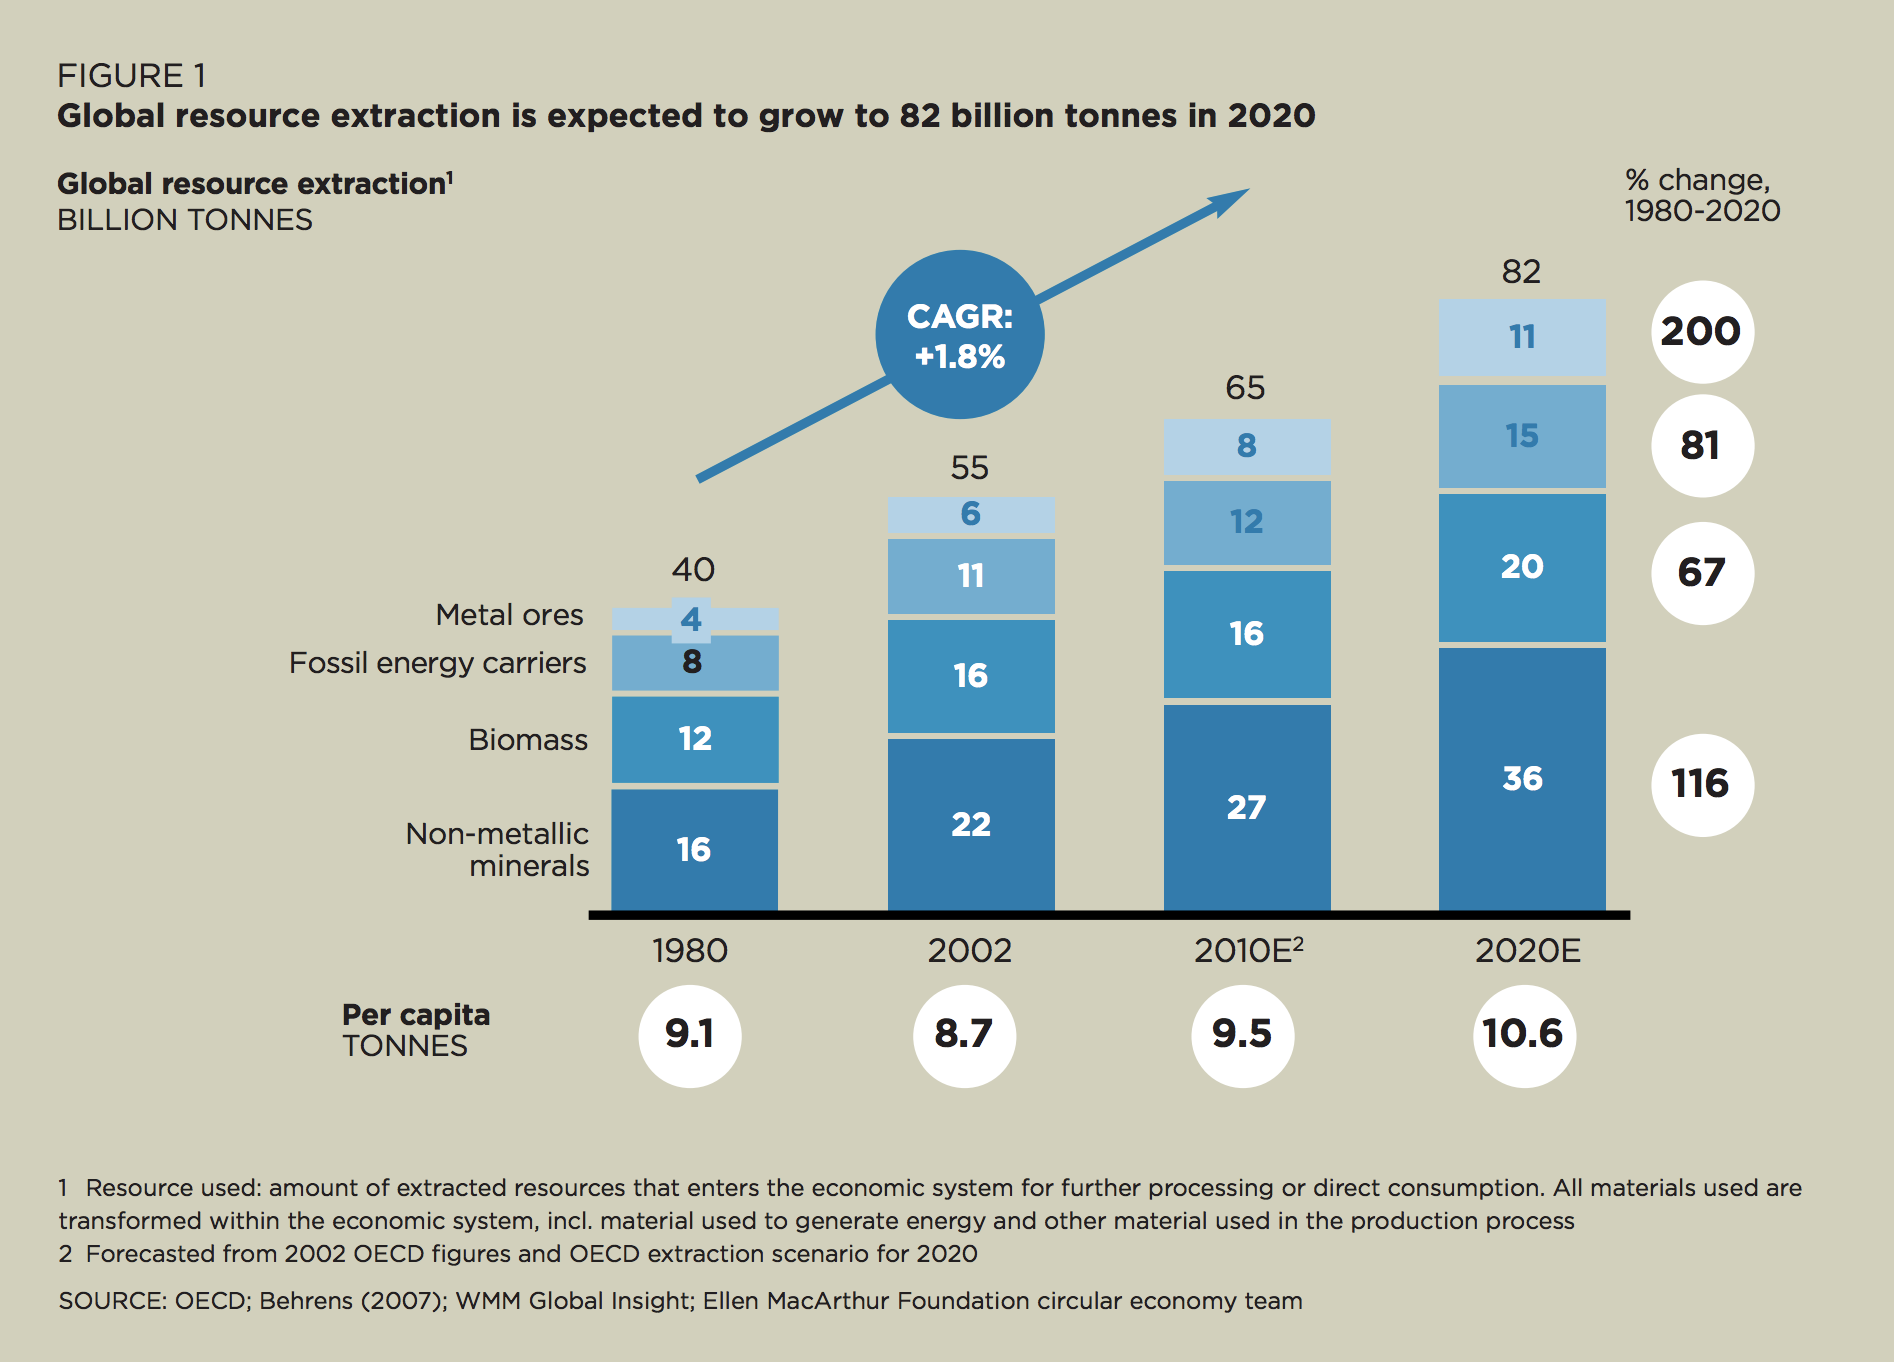
\includegraphics[height=0.7\textheight]{figures/mcarthur_extr.png}
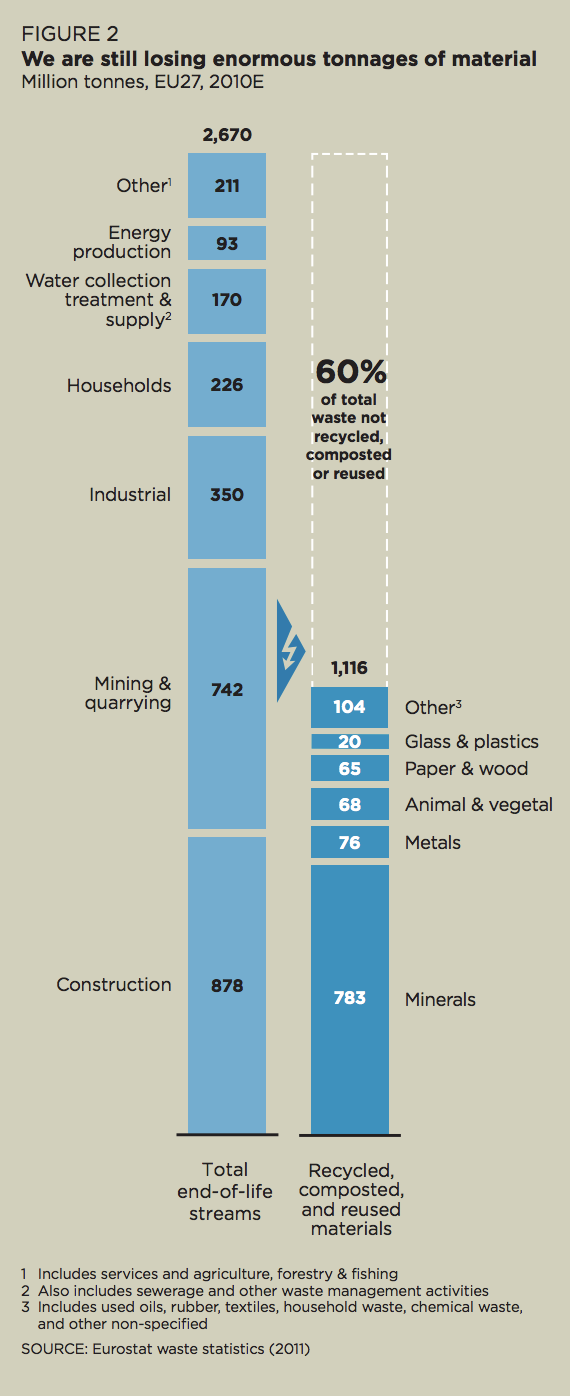
\includegraphics[height=0.7\textheight]{figures/mcarthur_recycl.png}
\end{center}

\tiny

MacArthur, E. (2013). Towards the circular economy. Journal of Industrial Ecology, 2, 23-44.

}

\sframe{Towards a circular economy}{

\begin{center}
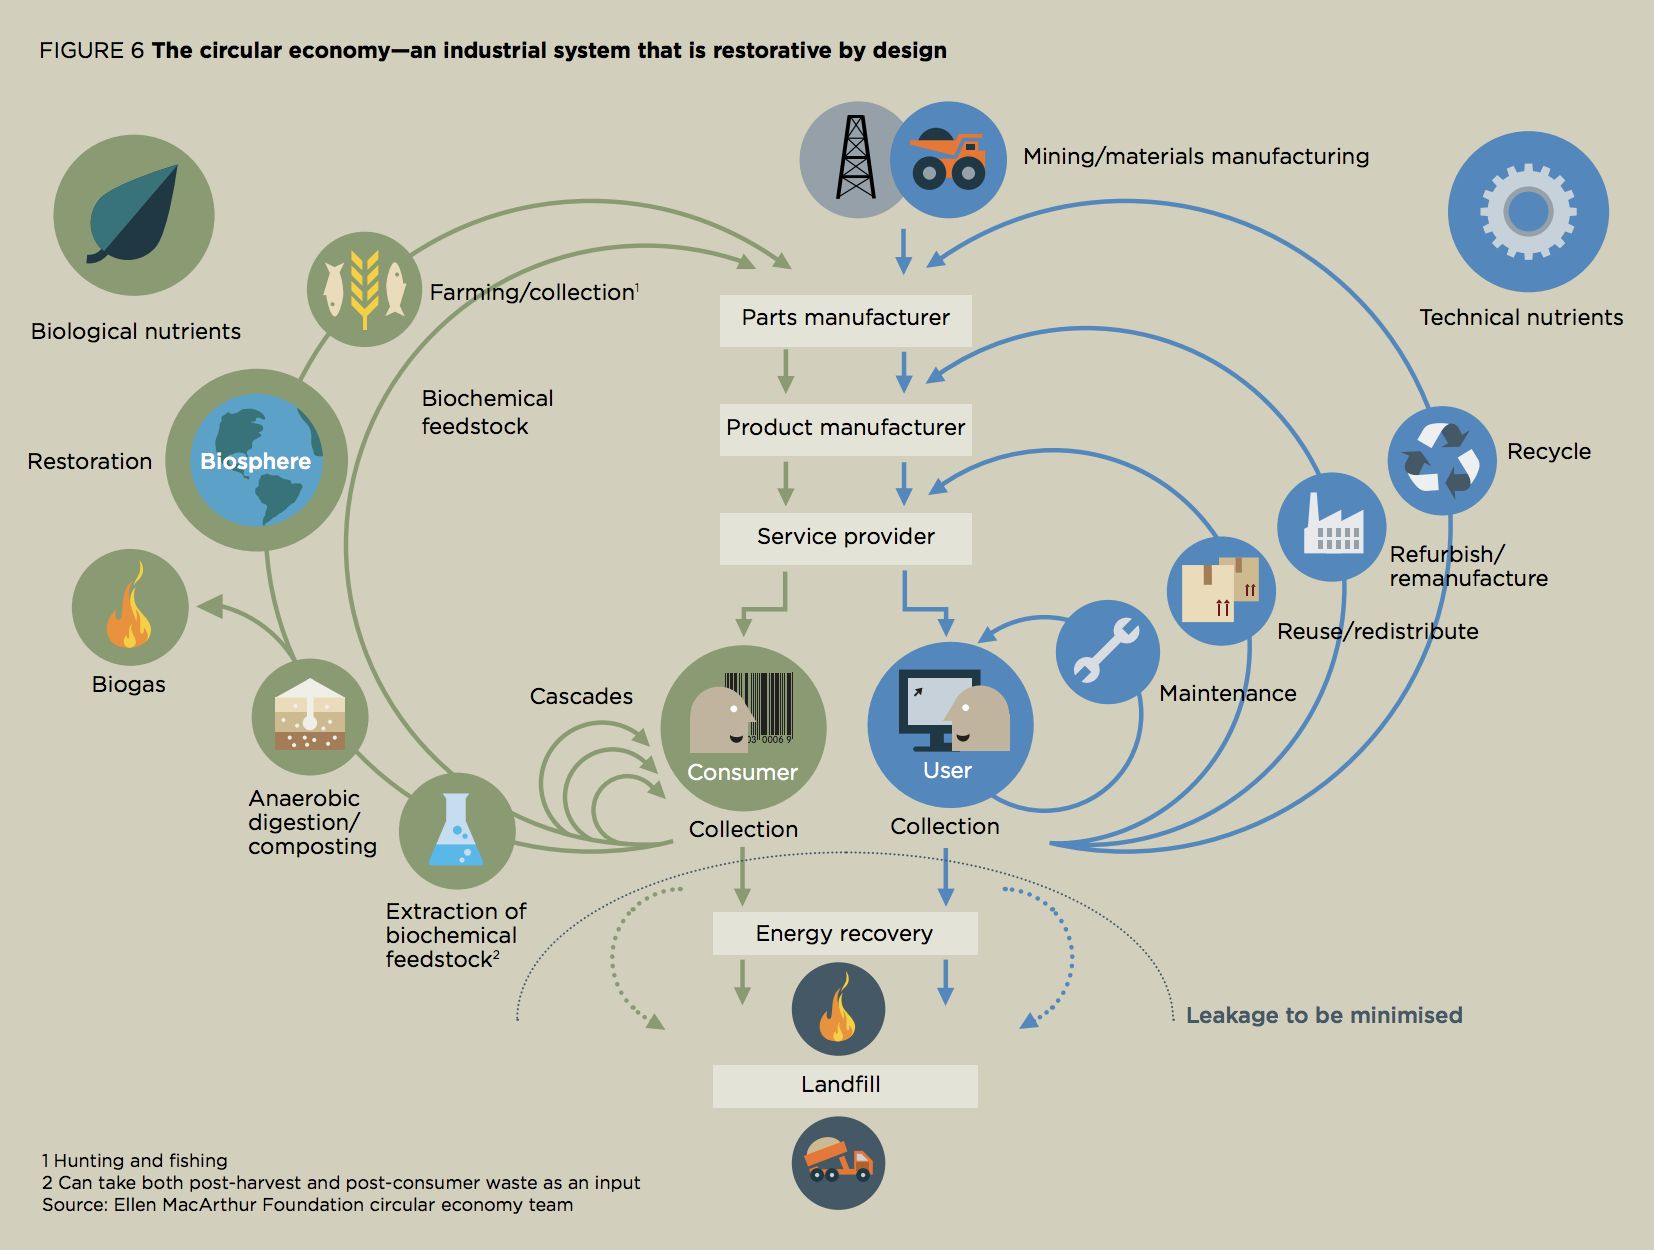
\includegraphics[height=0.8\textheight]{figures/mcarthur_circeco.png}
\end{center}

\footnotesize

\cite{macarthur2013towards}

%MacArthur, E. (2013). Towards the circular economy. Journal of Industrial Ecology, 2, 23-44.


}


\sframe{Industrial symbiosis}{

\textbf{Industrial symbiosis} as an approach to cycle by-products and energy between industries \cite{chertow2000industrial}, such as in eco-industrial parks

\cite{gibbs2007reflections}

\medskip

\begin{center}
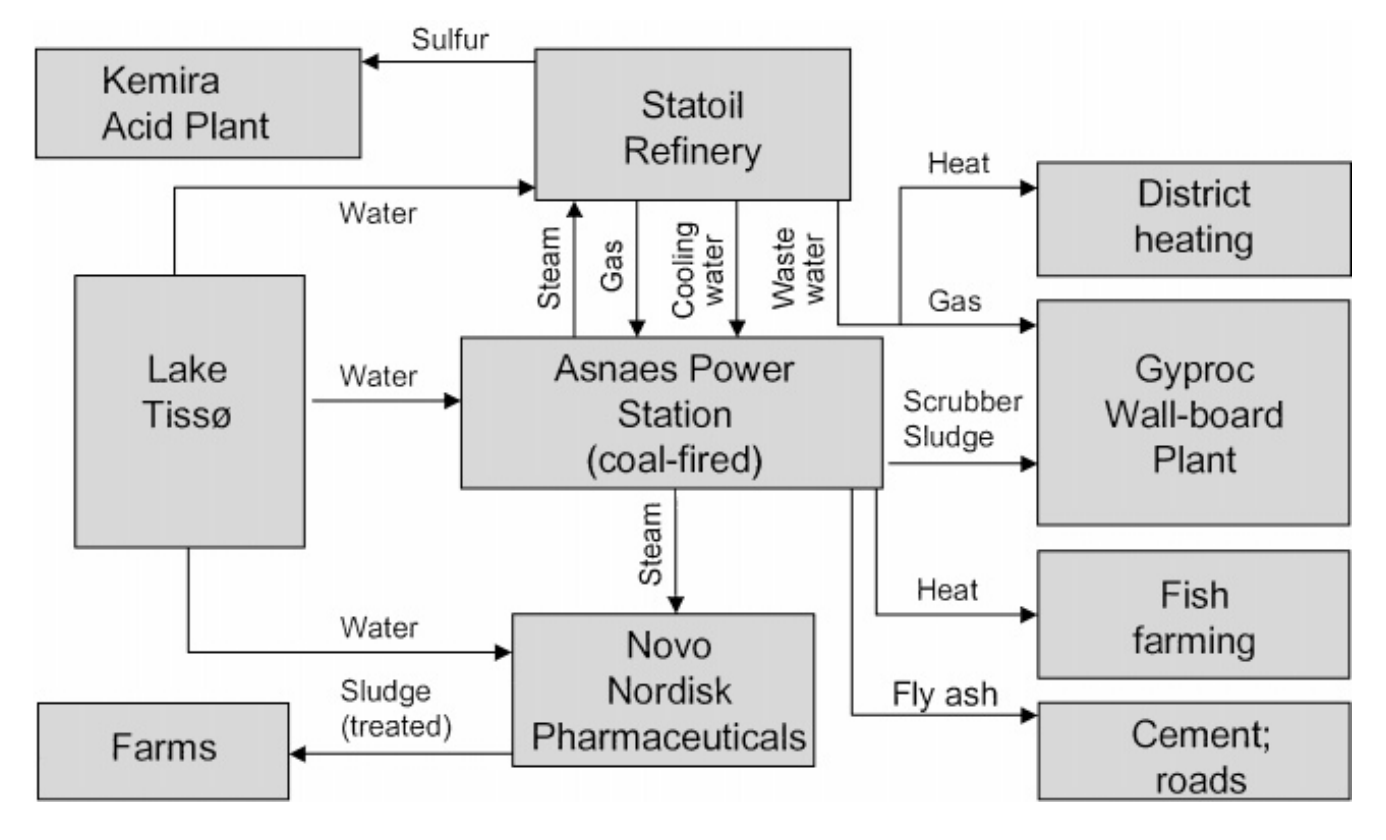
\includegraphics[width=0.7\linewidth]{figures/chertow_kalunborg.png}
\end{center}

\footnotesize

Chertow, M. R. (2000). Industrial symbiosis: literature and taxonomy. Annual review of energy and the environment, 25(1), 313-337.


}


\sframe{Industrial symbiosis and spatial structure}{

\justify



\textbf{Systems perspective} necessary to understand and optimize industrial symbiosis processes \cite{chertow2012organizing}

\bigskip


\textbf{Spatial structure} of the system plays a crucial role \cite{desrochers2001cities}

\bigskip

\textbf{Agent-based modeling} as a privileged modeling approach but never applied at regional scales from an urban system perspective 

\cite{kraines2006applying}

}


\sframe{An agent-based model for industrial symbiosis}{

$\rightarrow$ A simple agent-based model to study the effects of geographical proximity on industrial symbiosis network, and the role of cluster policies.

\medskip

$\rightarrow$ Integrates geography, ecology and economy concepts, from a generative social science perspective.

\medskip

$\rightarrow$ Can be applied to understand the interplay between different processes, and to optimize policies for a circular economy


\medskip

\begin{center}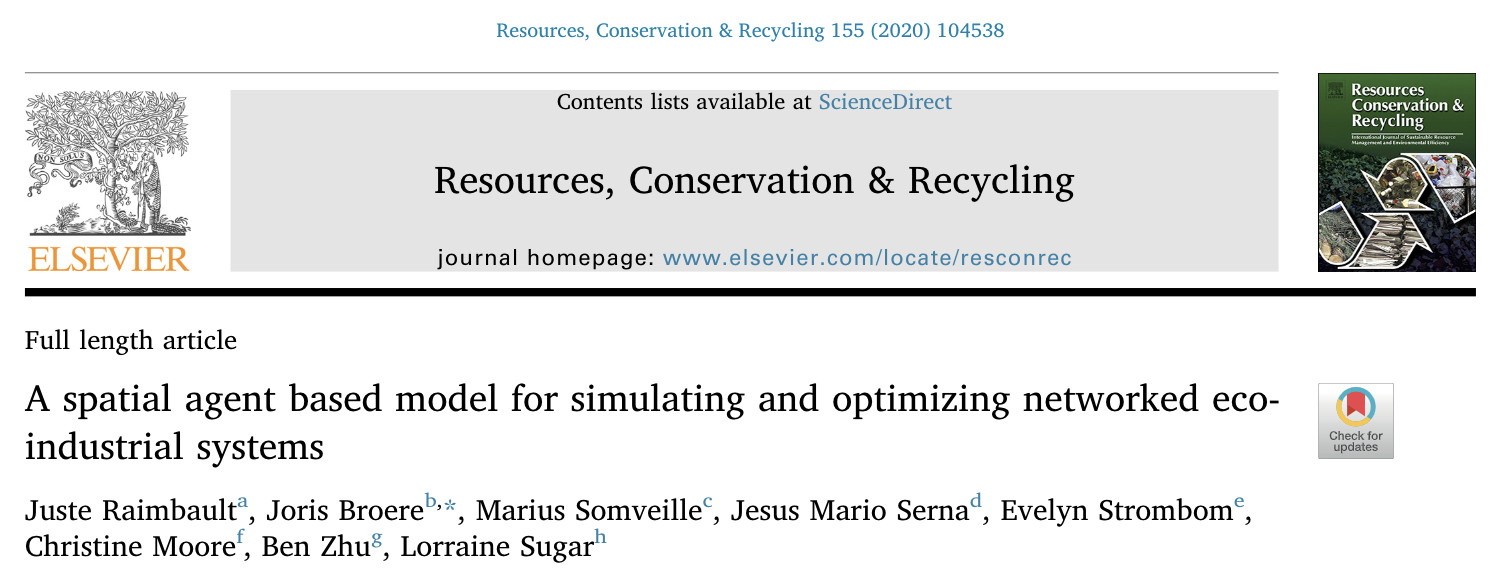
\includegraphics[width=0.9\textwidth]{figures/paper.png}
\end{center}


}

\sframe{Artificial life and generative models}{

\begin{center}
	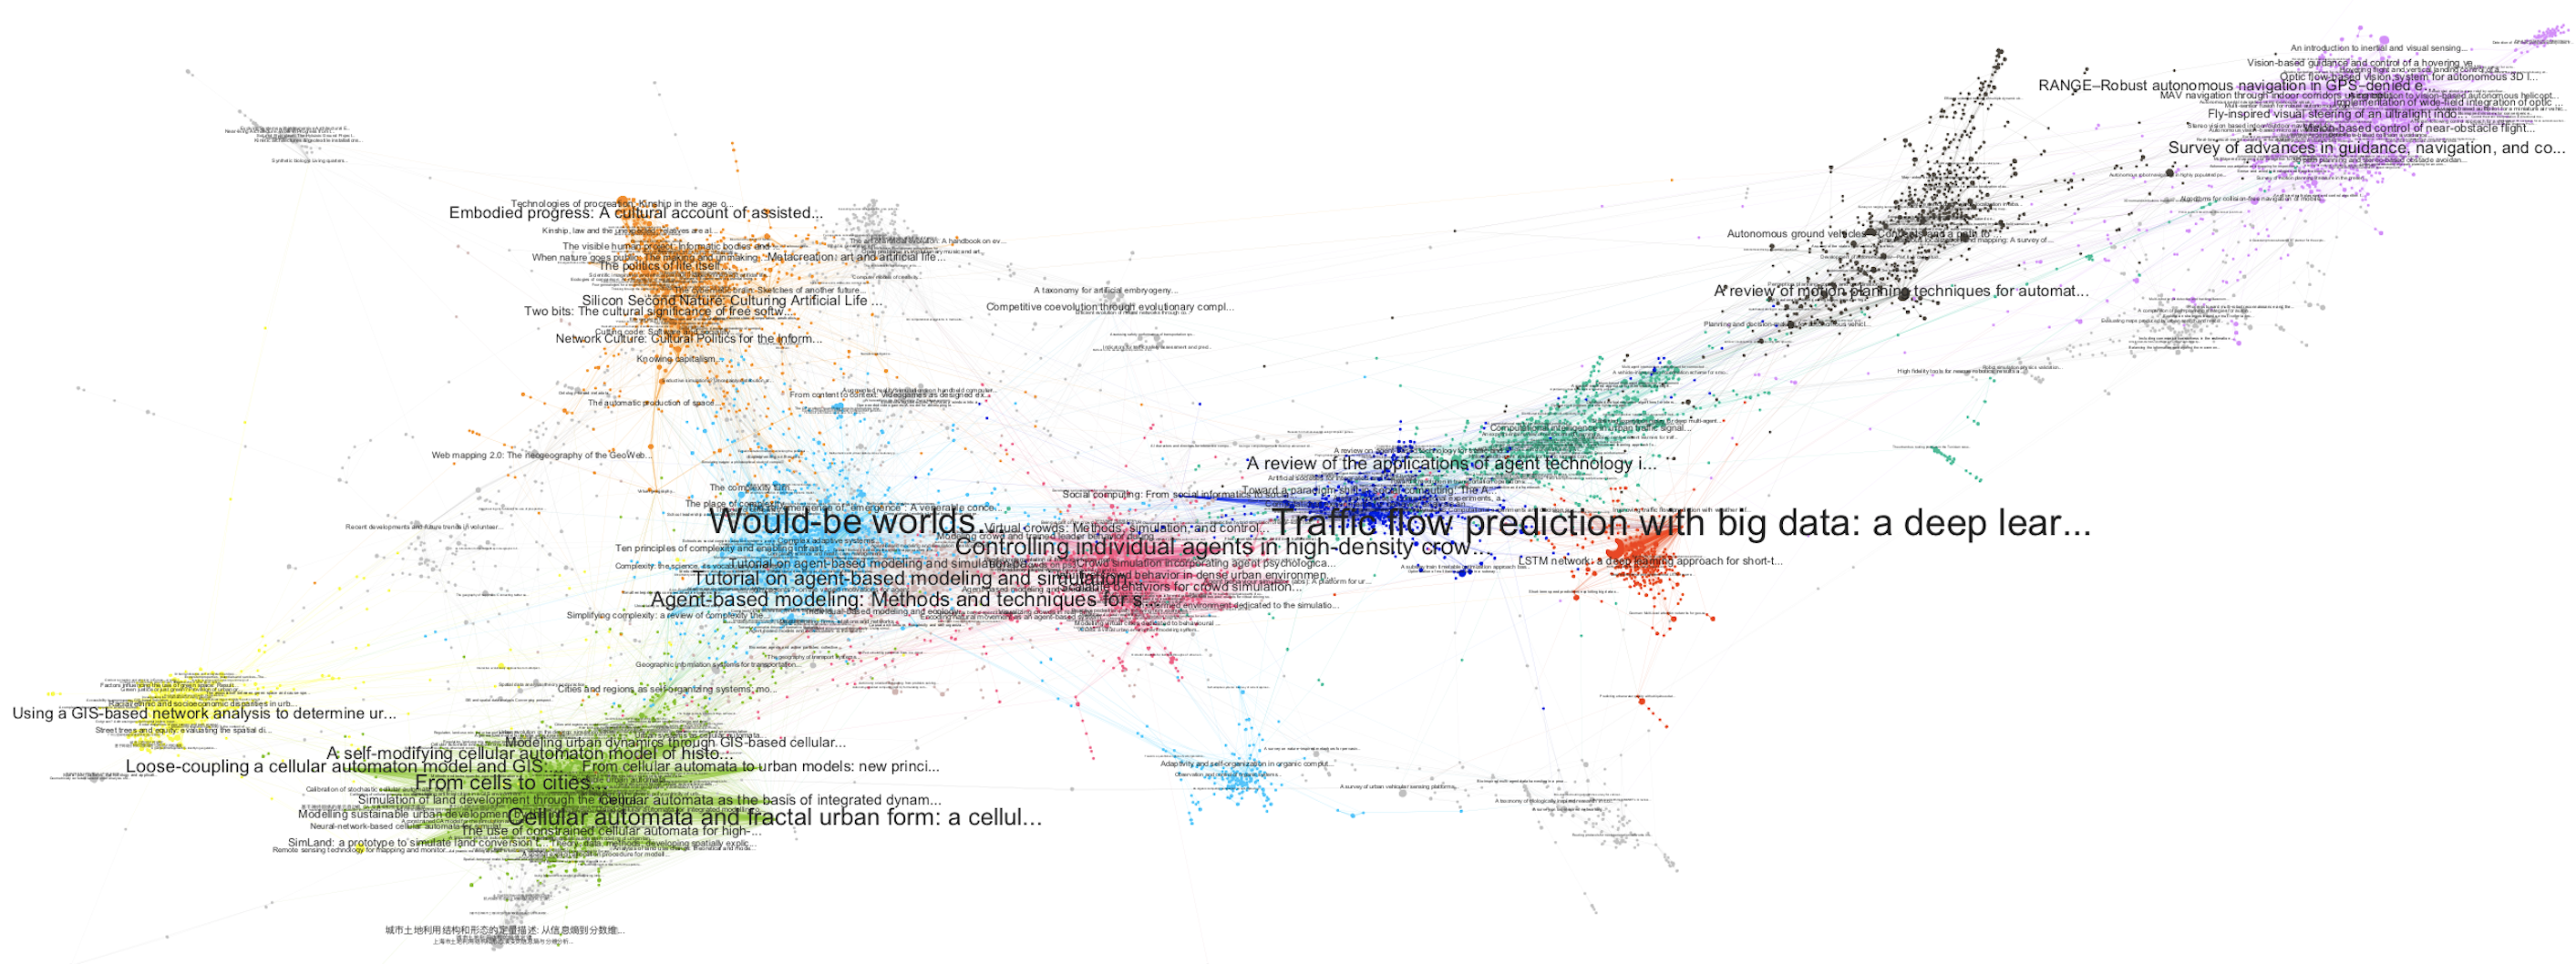
\includegraphics[width=\linewidth]{figures/corealife_zoom.png}
\end{center}

{\footnotesize \textit{Citation network of ALife studies of urban systems} \cite{raimbault2020cities} arXiv:2002.12926}

\medskip

\textbf{Transfer of concepts: } Urban morphogenesis, bio-inspired design, urban ecology, autopoiesis \cite{batty2009centenary}


\medskip

\textbf{Generative social science: } generating an emerging phenomenon from the bottom-up provides explanations \cite{epstein2006generative}



}

\section{Model description}


\sframe{Model summary}{

\begin{center}
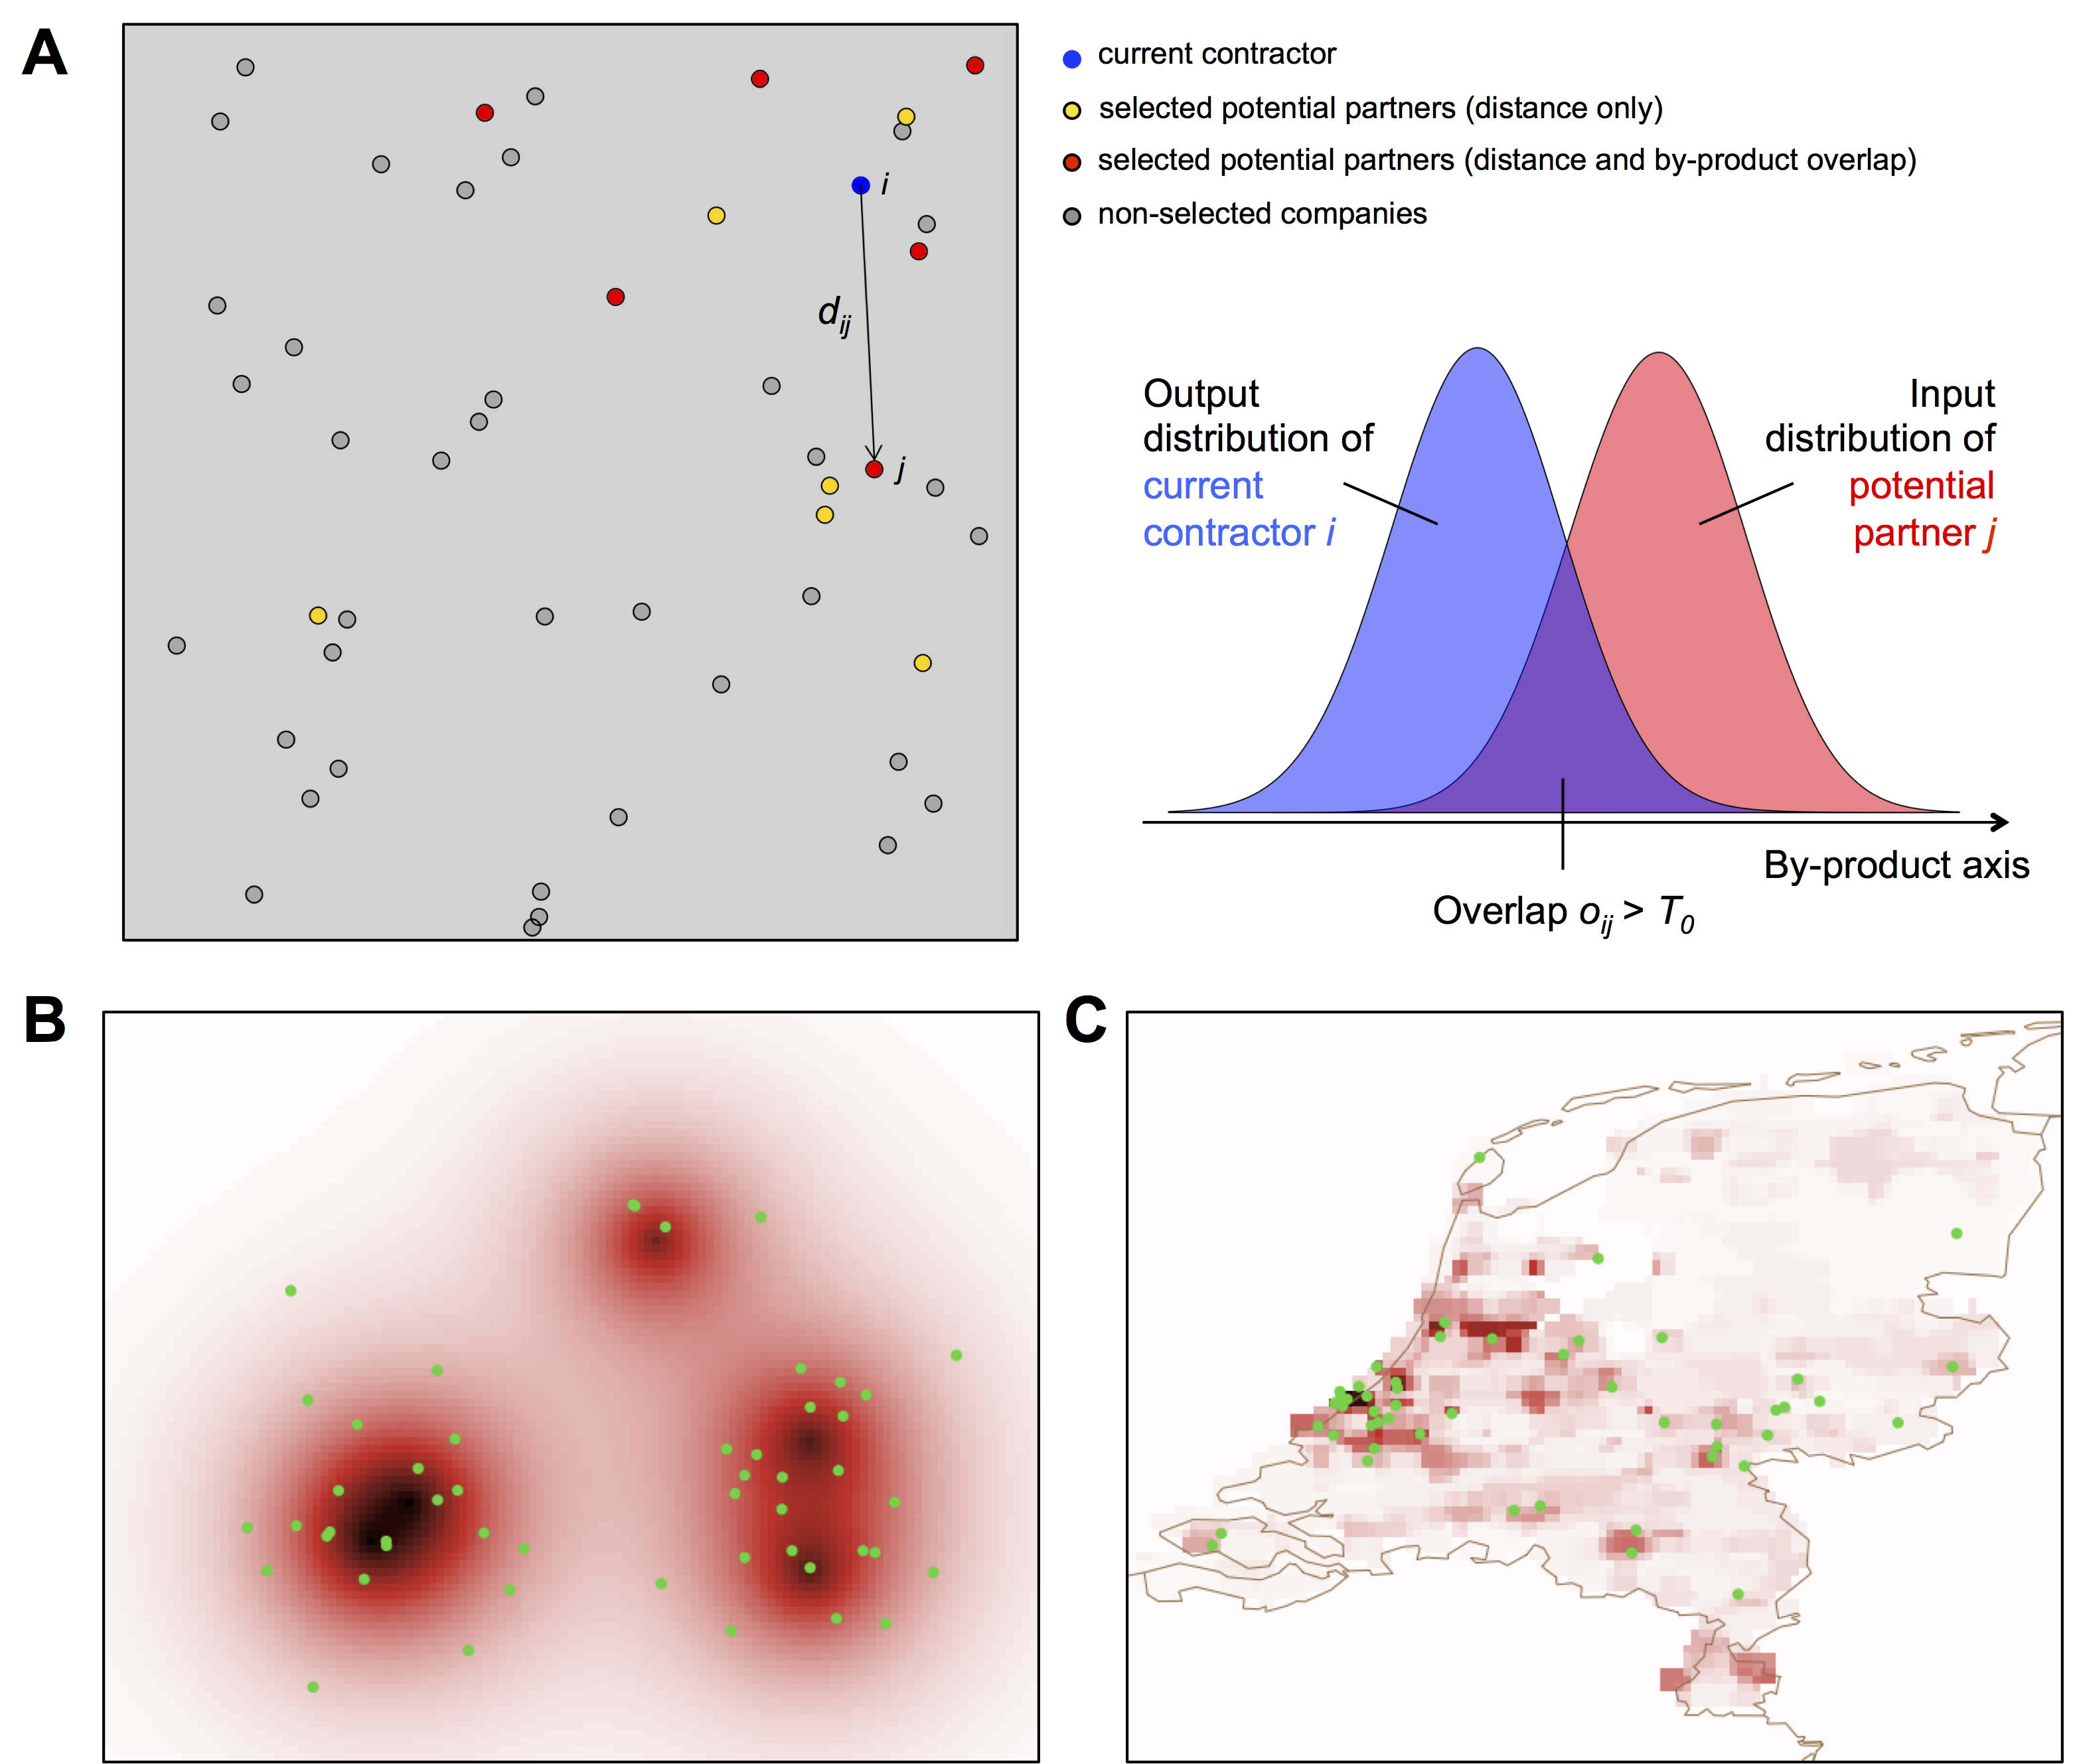
\includegraphics[height=0.85\textheight]{figures/Fig1.png}
\end{center}

}

\sframe{Model description}{

\textbf{Setup: } Companies located into space (synthetic or real setup), with input/output product distribution (Probabilistic Niche Model) which average is correlated with a clustering parameter $\alpha$

\medskip

\textbf{Network growth: } At each time step,
\begin{enumerate}
	\item A current contractor is drawn among companies with minimal number of links.
	\item Spatial interaction model (span $d_0$) determines potential partners.
	\item Partner with the best utility (linear in product overlap and transportation cost) is chosen, link created and distributions updated.
\end{enumerate}

\medskip 

Iterate until the network stabilizes. 

\medskip

\textbf{Indicators: } Total remaining waste (non exchanged products) and relative cost (network length weighted by flows).

}

\sframe{Processes and parameters}{

\begin{center}
\footnotesize
	\begin{tabular}{|l|l|l|l|l|l|}
	\hline
	Parameter & Notation & Process & Range & Value \\ \hline
	Number of firms & $N$ & Economic system & $\left[2 ; 10^6\right]$ & $N \textrm{ = } 50$\\ 
	Hierarchy of city system & $\gamma$ & City system & $\left[0.5 ; 2.0\right]$ & $\gamma \textrm{ = } 1.3$ \\ 
	Density-to-firms exponent & $\alpha_P$ & Economic system & $\left[0.1 ; 4.0\right]$ & $\alpha_P \textrm{ = } 1.5$ \\
	Number of centers & $p$ & City system & $\left[1 ; 10\right]$ & $p \textrm{ = } 5$  \\\hline
	Gravity decay & $d_0$ & Spatial interactions & $\left[1;200\right]$ & $d_0 \textrm{ = } 50 km$ \\
	Distribution width & $\sigma$ & Industrial structure & $\left[0.01 ; 0.1\right]$ & $\sigma \textrm{ = } 0.05$ \\
	Overlap threshold & $T_0$ & Industrial structure & $\left[0.01 ; 0.1\right]$ & $T_0 \textrm{ = } 0.1$ \\
	Transportation cost & $c$ & Urban system & $\left[0.1 ; 4.0\right]$ & $c \textrm{ = } 0.5$ \\
	Correlation level & $\alpha$ & Industrial clusters & $\left[0 ; 20.0\right]$ & $\alpha \textrm{ = } 5$ \\\hline
	\end{tabular}
		
\end{center}



}



\section{Results}

\sframe{Examples of generated networks}{

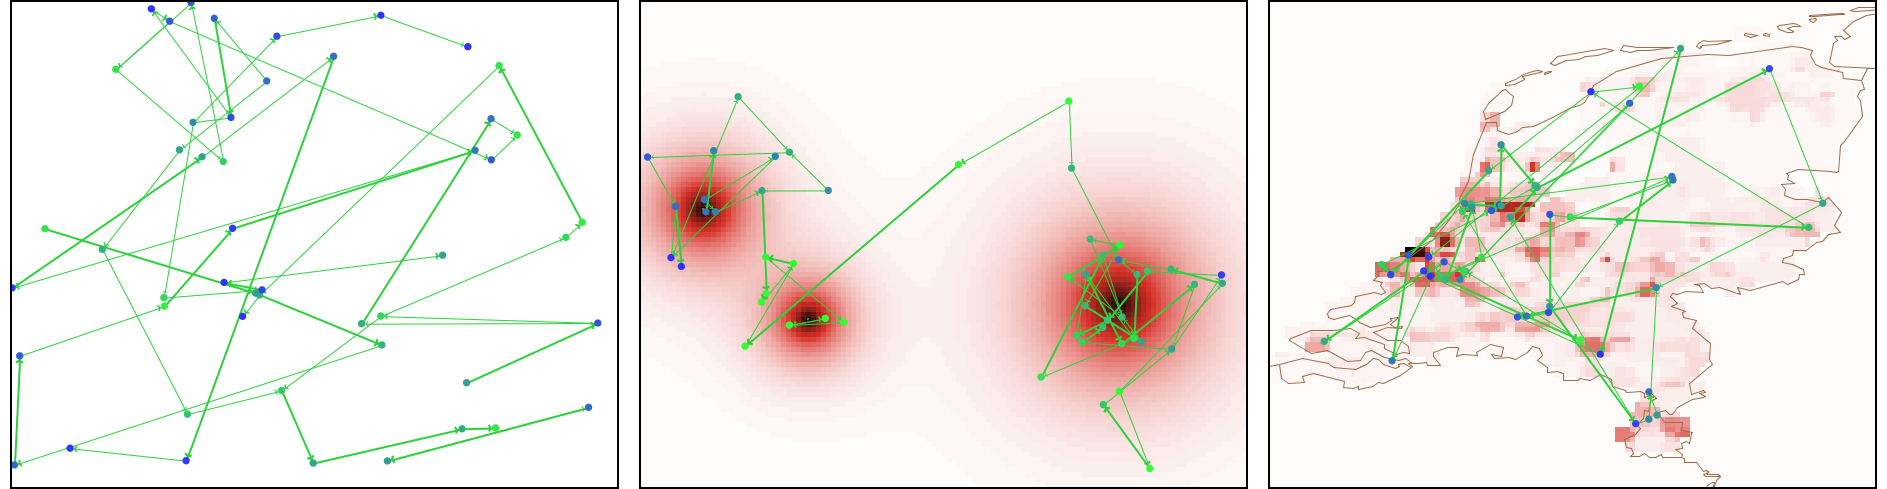
\includegraphics[width=\textwidth]{figures/Fig2.png}

\medskip

\textit{Random company positions, synthetic urban system (scaling law of population), and real population distribution.}

\medskip

\textbf{Model demonstration}


}


\sframe{Model implementation and exploration}{

\justify

\textit{Spatial model with several parameters}

$\rightarrow$ model implemented in NetLogo for its compromise between performance and interactivity

\bigskip

\textit{Consequent number of parameters and processes}



$\rightarrow$ integration into the OpenMOLE model exploration open source software \cite{reuillon2013openmole} 

\url{https://next.openmole.org}

\bigskip

\begin{center}

\includegraphics[height=0.13\textheight]{figures/iconOM.png}

\includegraphics[height=0.13\textheight]{figures/openmole.png}
\end{center}



\textit{Enables seamlessly (i) model embedding; (ii) access to HPC resources; (iii) exploration and optimization algorithms}


}


\sframe{Baseline behavior of the model}{

Running grid sampling on synthetic urban systems with no correlation process:

\begin{itemize}
	\item Statistical consistency of indicators, $n\textrm{=}100$ replications fixed for following experiments.
	\item Expected effect of some parameters, in particular company product span $\sigma$ (decreases waste) and transportation cost $c$ (increases waste and decreases relative cost).
	\item Emerging behaviors: congestion effect with $T_0$ exchange threshold; U-shaped behavior of cost as a function of $\sigma$.
	\item Different qualitative patterns between synthetic and real system for company position setup.
\end{itemize}


}


\sframe{Policy optimization for the circular economy}{

\begin{center}
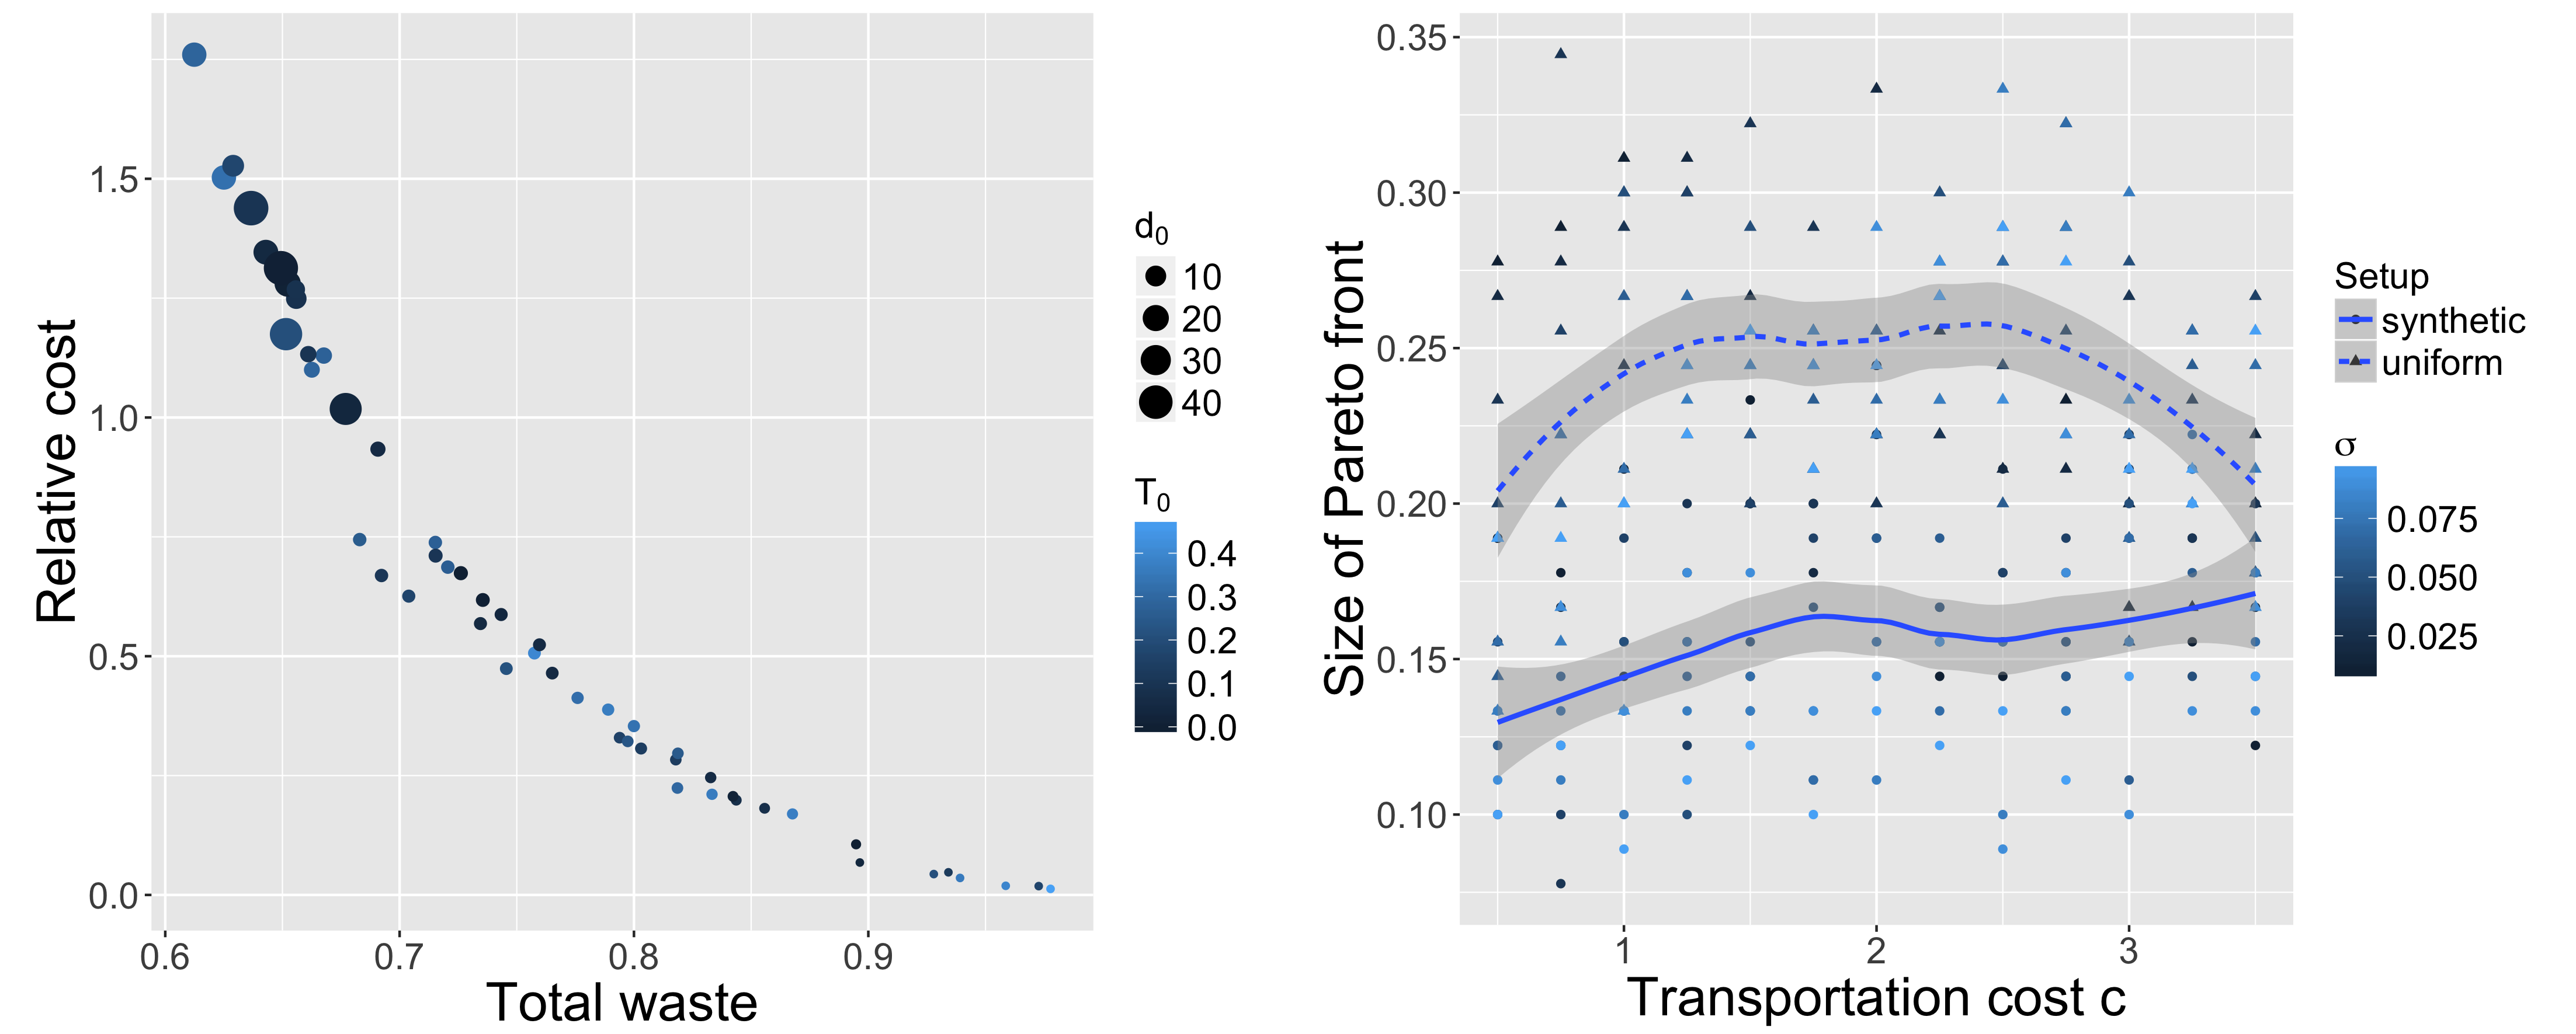
\includegraphics[width=\textwidth]{figures/Fig3.png}
\end{center}

\medskip

\textit{(Left) At fixed exogenous parameters $c$ and $\sigma$, bi-objective optimization of cost and waste; (Right) Size of Pareto fronts (number of alternatives for policy optimization) as a function of $c$ and $\sigma$.}

}


\sframe{Spatial correlation between inputs and outputs}{

\begin{center}
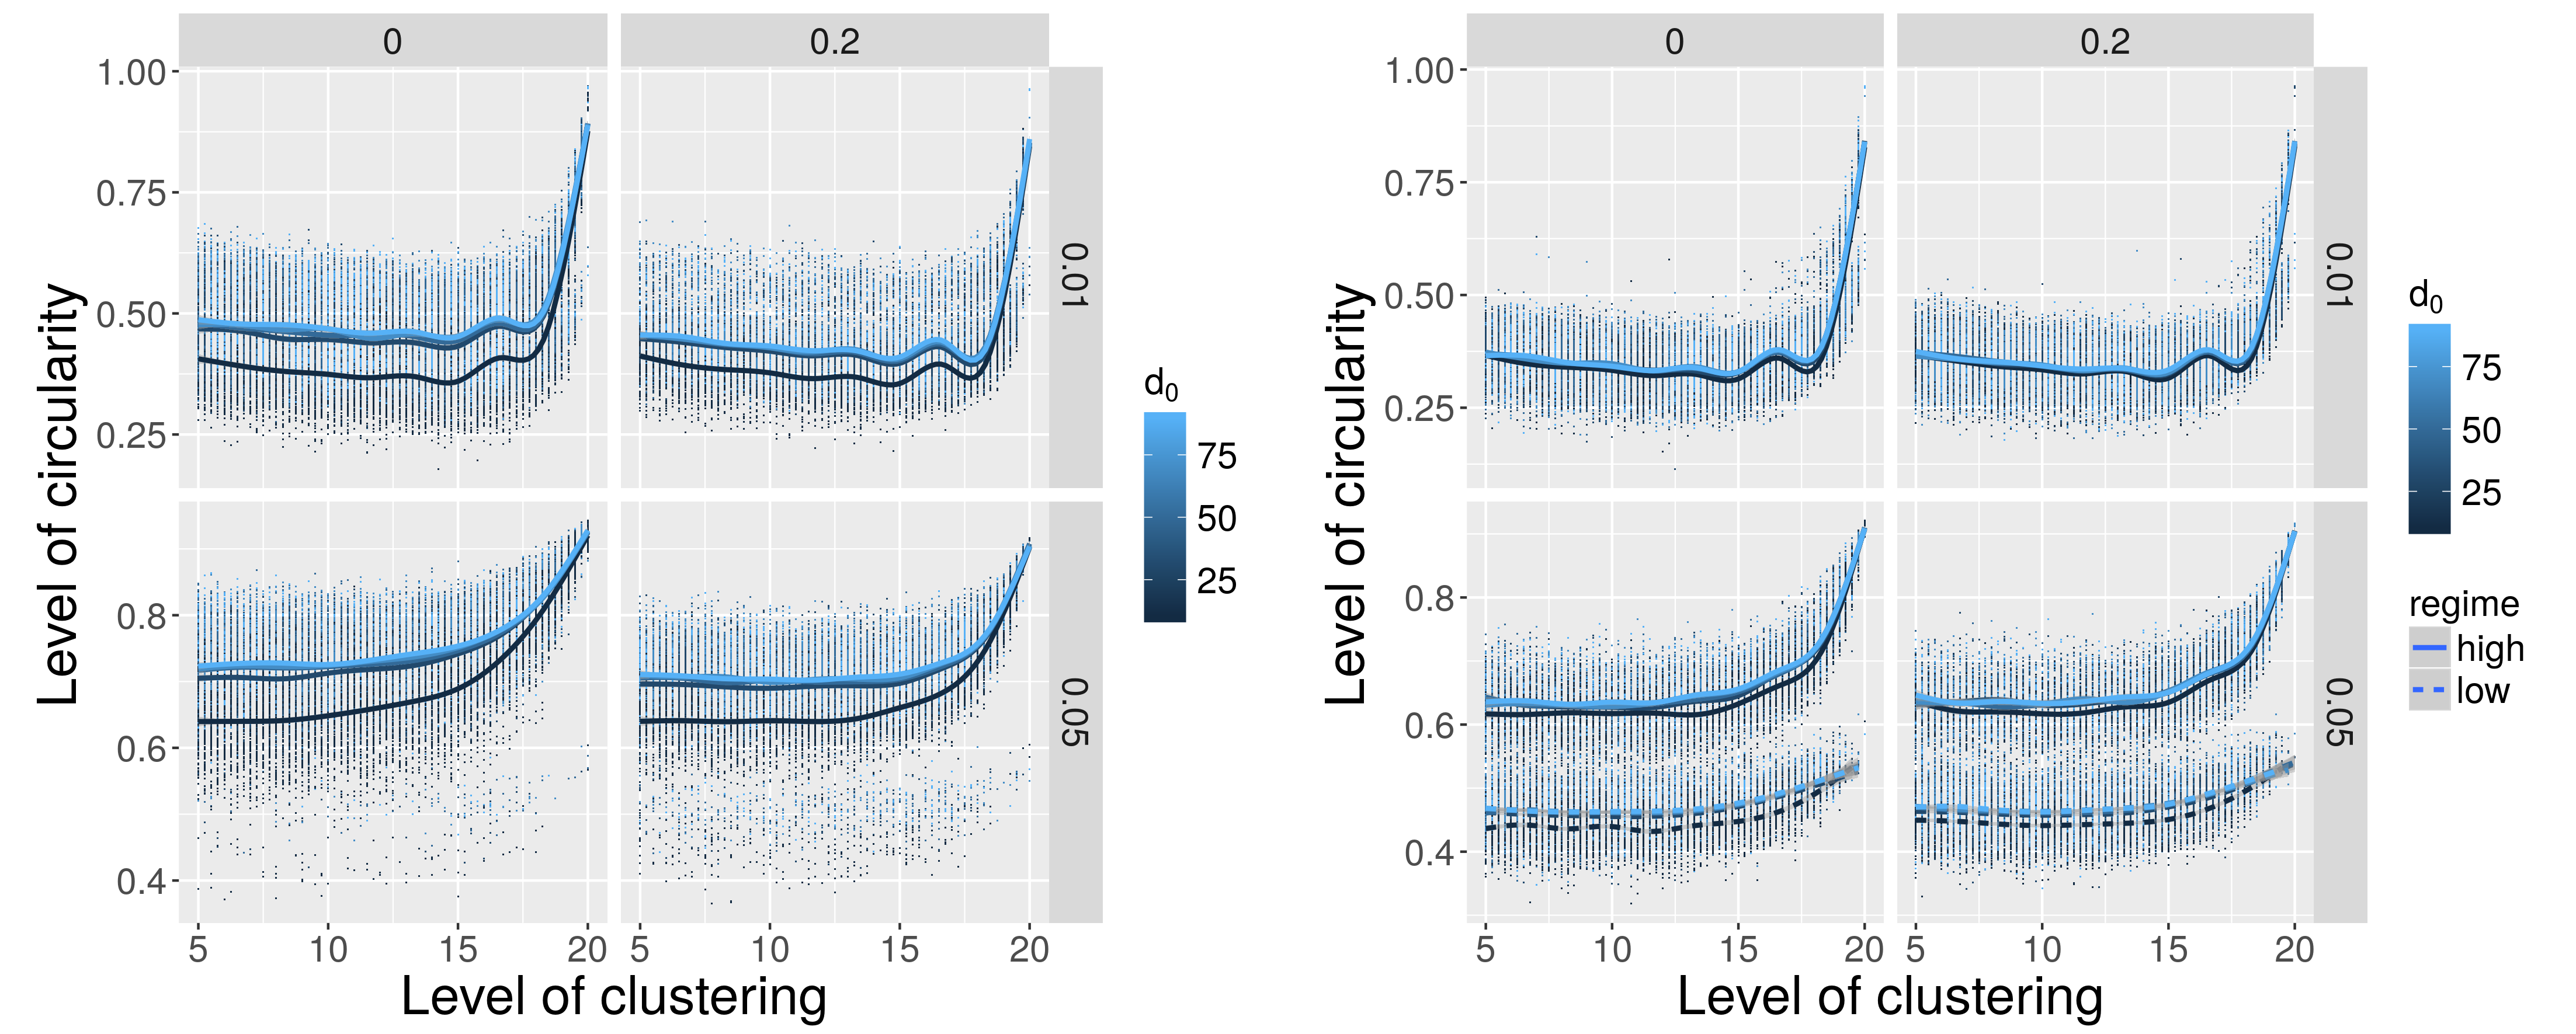
\includegraphics[width=\textwidth]{figures/Fig4.png}
\end{center}

\medskip
\footnotesize

\textit{Influence of level of clustering on the circularity of the final network, for low (resp. high) transportation cost (Left, resp. Right), for different thresholds $T_0$ (columns), distribution width $\sigma$ (rows) and gravity decay $d_0$ (color).}

$\rightarrow$ In practice, the spatial correlation policy must be strictly enforced to have an effect.

}

\sframe{Model calibration}{

\begin{center}
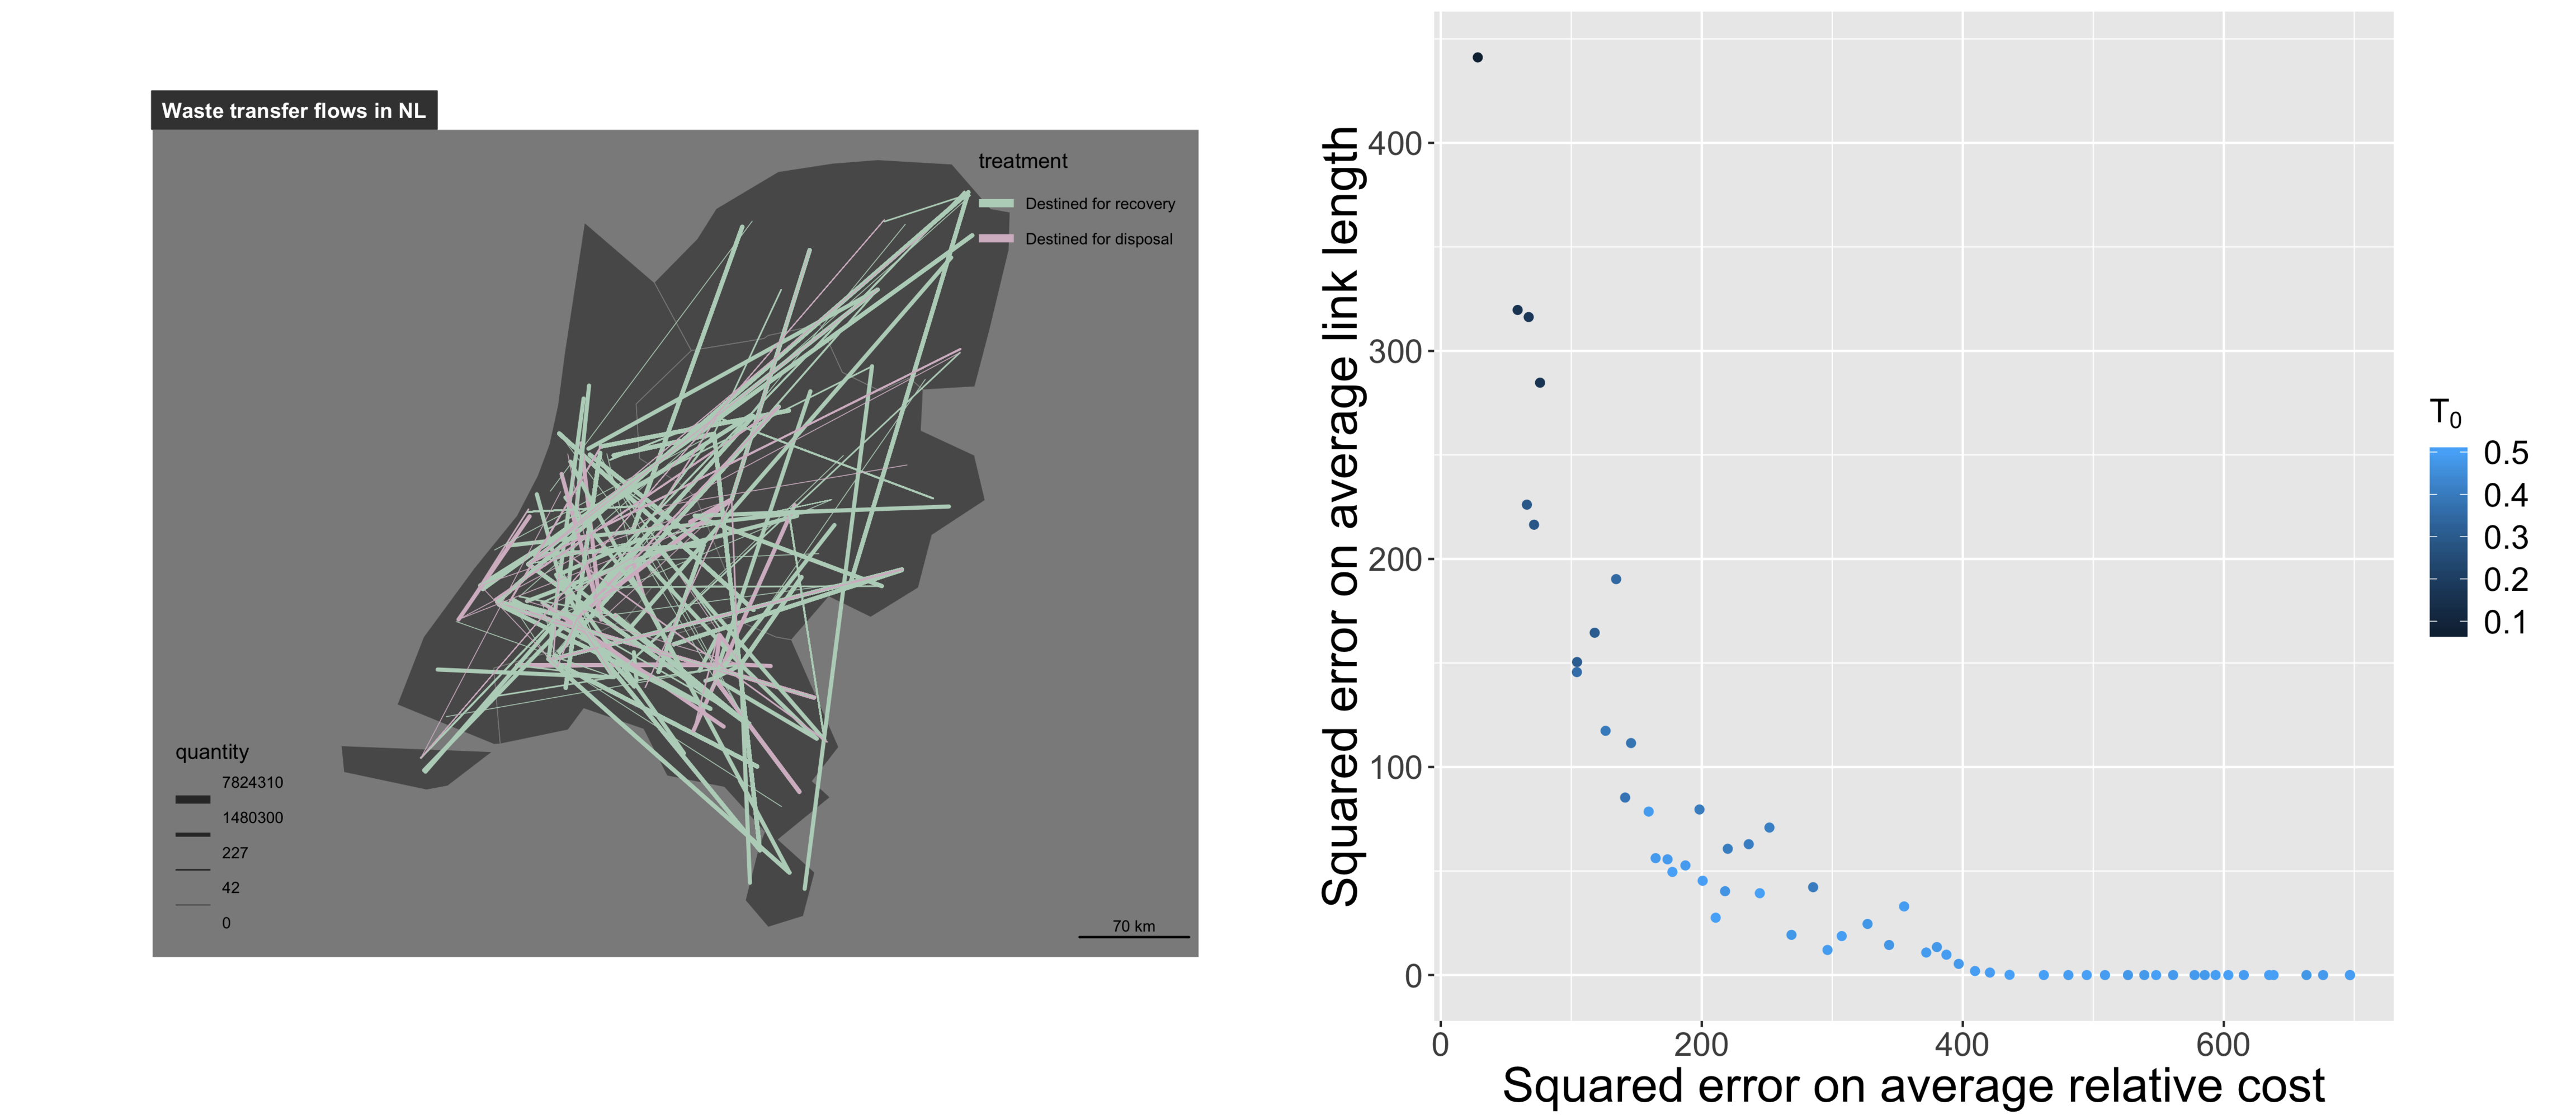
\includegraphics[width=\textwidth]{figures/Fig5.png}
\end{center}

\medskip
\footnotesize

\textit{Real-world application of the model by calibration on the EPRTR database to reproduce network structure (number of links, average link length, relative cost); yield medium range interactions but high propensity to exchange.}

}



\section{Discussion}

\sframe{Discussion}{

\textbf{Implications}

\medskip

$\rightarrow$ Importance of spatial configuration; Eco-industrial park policies must be strictly applied.

\medskip

$\rightarrow$ Real-world application of the model shown as a proof-of-concept with good model fit.

\bigskip

\textbf{Developments}

\medskip

$\rightarrow$ Data-driven approach in link with an interactive web application: towards a real-world application with a project of company.

\medskip

$\rightarrow$ Refinement of economic processes.

\medskip

$\rightarrow$ Benchmark of multiple possible processes and levels of policies.


}



\sframe{Conclusion}{


$\rightarrow$ A simple agent-based model to understand and optimize industrial symbiosis.

\medskip

$\rightarrow$ Important role of spatial structure and spatial correlations.


\bigskip
\bigskip

\footnotesize

\textbf{Git repository: } \texttt{https://github.com/SFICSSS16-CircularEconomy/CircularEconomy}

\bigskip

\textbf{Simulation data: }\texttt{https://doi.org/10.7910/DVN/7XCWTN}% dataverse


\bigskip

\textbf{Acknowledgments}: thanks to the \textit{European Grid Infrastructure} for access to the infrastructure.


}



%%%%%%%%%%%%%%%%%%%%%
\begin{frame}[allowframebreaks]
\frametitle{References}
\bibliographystyle{apalike}
\bibliography{biblio}
\end{frame}
%%%%%%%%%%%%%%%%%%%%%%%%%%%%










\end{document}

